 \documentclass[11pt, oneside]{article}   	% use "amsart" instead of "article" for AMSLaTeX format
\usepackage{geometry}                		% See geometry.pdf to learn the layout options. There are lots.
\geometry{letterpaper}                   		% ... or a4paper or a5paper or ... 
%\geometry{landscape}                		% Activate for for rotated page geometry
%\usepackage[parfill]{parskip}    		% Activate to begin paragraphs with an empty line rather than an indent
\usepackage{graphicx}				% Use pdf, png, jpg, or eps� with pdflatex; use eps in DVI mode
								% TeX will automatically convert eps --> pdf in pdflatex		
\usepackage{amssymb}
\usepackage{amsmath}
\usepackage{parskip}
\usepackage{color}
\usepackage{hyperref}

\title{Cauchy integral theorem}
%\author{The Author}
%\section{}
%\subsection*{}
\date{}							% Activate to display a given date or no date

\graphicspath{{/Users/telliott_admin/Dropbox/Tex/png/}}
% \begin{center} 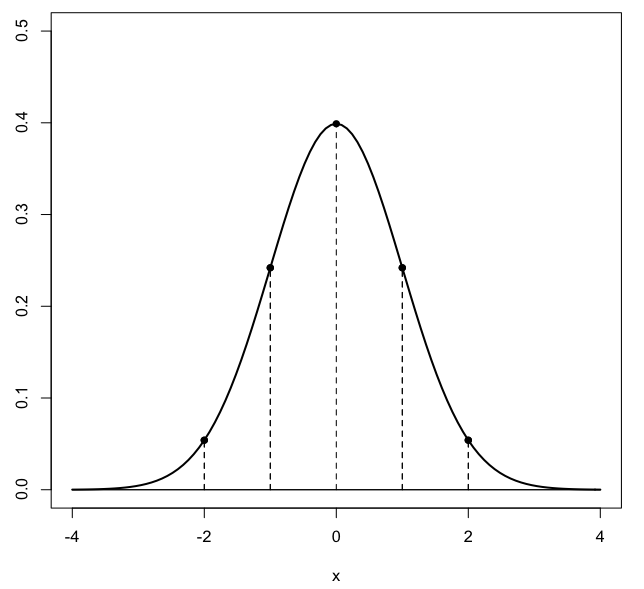
\includegraphics [scale=0.4] {gauss3.png} \end{center}
\begin{document}
\maketitle
\Large

\subsection*{derivation of Cauchy 2}
Suppose $f(z)$ is analytic everywhere within some region \emph{except} at a singularity, $z_0$.  For example, suppose we have
\[ \frac{f(z)}{z-z_0} \]
and suppose we integrate this around a special closed path in the region of analyticity:
\[ \oint \frac{f(z)}{z-z_0} \ dz \]
\begin{center} 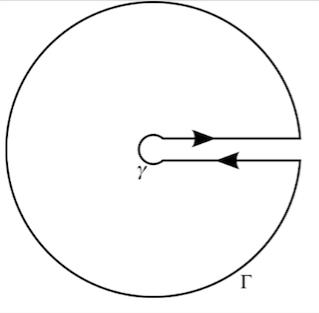
\includegraphics [scale=0.6] {keyhole.png} \end{center}
It's not labeled but the singularity $z_0$ is at the center of the two concentric circles.  The "keyhole" excludes $z_0$ so $f$ is analytic everywhere in the region enclosed by the path, and the total integral is zero by Cauchy's first theorem.  The straight line segments are so close as to be equal, but traversed in opposite directions, so the contribution from them is zero.  Thus we have that the integral around the outer ring counter-clockwise + the integral around the inner ring clockwise add up to zero.

Reversing the direction of integration on the inner ring changes the sign of the value, hence we have that
\[ \oint_{C \ \text{outer}} \frac{f(z)}{z-z_0} \ dz - \oint_{C \ \text{inner}} \frac{f(z)}{z-z_0} \ dz = 0 \]
But we haven't said anything about the radius of these rings.  

What this means is that the value of the integral around a ring enclosing a singularity is not zero, but it has the same value for a ring of \emph{any} radius.  It's independent of the radius.
\[ \oint_{C \ \text{outer}} \frac{f(z)}{z-z_0} \ dz = \oint_{C \ \text{inner}} \frac{f(z)}{z-z_0} \ dz \]

We can parametrize this path by saying that each point on the curve is given by
\[ z = z_0 + \rho e^{i\theta}, \ \ \ 0 \le \theta \le 2 \pi \]
\[ dz = \rho i e^{i \theta} \ d \theta \]
\[ \oint \frac{f(z)}{z - z_0} \ dz = \int_0^{2\pi} \frac{f(z_0 + \rho e^{i\theta})}{\rho e^{i \theta}} \ \rho i e^{i\theta} \ d \theta \]
\[ = i \int_0^{2\pi}  f(z_0 + \rho e^{i\theta}) \ d \theta \]
\[ = i \int_0^{2\pi}  f(z) \ d \theta \]
We may choose $\rho$ as small as we like, and so we choose it very small ($\rho \rightarrow 0$) so
\[ f(z) \rightarrow f(z_0) = \text{constant} \]
and since it's constant we can bring it out of the integral!
\[  \oint \frac{f(z)}{z - z_0} \ dz = f(z_0) i \int_0^{2\pi} d \theta \]
\[ = 2 \pi i f(z_0) \]

\subsection*{using Cauchy 2}
Example:  consider a semicircle of radius $R$ lying in the first two quadrants with its diameter on the real $x$-axis, and a function.   We wish to evaluate:
\[ \oint_C f(z) \ dz \]
\[ = \oint_C \frac{e^{iaz}}{b^2 + z^2} \ dz \]
where $a$ and $b$ are positive constants.  $f(z)$ has singularities at $z = \pm ib$, where $b < R$.  In particular, we are interested in what happens as $R \rightarrow \infty$.

Along the $x$-axis, we have $y=0$ and $dy = 0$, so $dz = dx$ and
\[ \int_{C1} = \int_{-R}^R \frac{e^{iax}}{b^2 + x^2} \ dx \]
Along the semi-circular arc, we have $r = R$ and $\theta = 0 \rightarrow \pi$ and
\[ z = Re^{i\theta} \]
\[ dz = iRe^{i\theta} \ d \theta \]
\[ \int_{C2} = \int_0^{\pi}  \frac{e^{ia(Re^{i\theta})}}{b^2 + R^2e^{i2\theta}}  \ iRe^{i\theta} \ d \theta \]
Thus
\[ \oint_C z \ dz = \oint_C \frac{e^{iaz}}{b^2 + z^2} \ dz \]
\[ = \int_{-R}^R \frac{e^{iax}}{b^2 + x^2} \ dx + \int_0^{\pi}  \frac{e^{ia(Re^{i\theta})}}{b^2 + R^2e^{i2\theta}}  \ iRe^{i\theta} \ d \theta \]

Rewriting the integrand for the integral on the left-hand side:
\[ \frac{e^{iaz}}{b^2 + z^2} = \frac{e^{iaz}}{(z + ib)(z - ib)} = \frac{e^{iaz}}{i2b} ( \frac{1}{z-ib} - \frac{1}{z+ib}) \]
Having factored out $1/i2b$, rewrite the integral as
\[ \frac{1}{i2b} \ (\oint \frac{e^{iaz}}{z-ib} \ dz - \oint \frac{e^{iaz}}{z + ib} \ dz) = \int_{-R}^R \frac{e^{iax}}{b^2 + x^2} \ dx + \int_0^{\pi}  \frac{e^{ia(Re^{i\theta})}}{b^2 + R^2e^{i2\theta}}  \ iRe^{i\theta} \ d \theta \]
That's quite a mouthful!

The second term on the left-hand side has a singularity at $z = -ib$, which is \emph{outside} the region (actually, below it) and hence by Cauchy 1 that integral is zero.

So now
\[ \frac{1}{i2b} \ \oint \frac{e^{iaz}}{z-ib} \ dz  = \int_{-R}^R \frac{e^{iax}}{b^2 + x^2} \ dx + \int_0^{\pi}  \frac{e^{ia(Re^{i\theta})}}{b^2 + R^2e^{i2\theta}}  \ iRe^{i\theta} \ d \theta \]

Looking at the other contour integral 
\[ \frac{1}{i2b} \ \oint \frac{e^{iaz}}{z-ib} \ dz  \]

we have a singularity at $z = z_0 = ib$, which, as $R$ becomes large, is inside the semicircular region and thus by Cauchy 2 the integral is equal to $2 \pi i \ f(z_0)$ where
\[ f(z_0) = e^{iaz_0} = e^{iaib} = e^{-ab} \]
and so we have
\[ \frac{1}{i2b} \ \oint \frac{e^{iaz}}{z-ib} \ dz = \frac{1}{i2b} 2 \pi i e^{-ab}, \ \ R > b \]
\[ = \frac{\pi}{b} e^{-ab} \]

Putting it all together
\[ \frac{\pi}{b} e^{-ab} = \int_{-R}^R \frac{e^{iax}}{b^2 + x^2} \ dx + \int_0^{\pi}  \frac{e^{ia(Re^{i\theta})}}{b^2 + R^2e^{i2\theta}}  \ iRe^{i\theta} \ d \theta \]
Nahin shows that the second integral on the right-hand side vanishes as $R \rightarrow \infty$.  This has gotten a bit out of hand so I will just assume that part and say then that:
\[ \frac{\pi}{b} e^{-ab} = \int_{-\infty}^{\infty} \frac{e^{iax}}{b^2 + x^2} \ dx \]\
\[ \frac{\pi}{b} e^{-ab} = \int_{-\infty}^{\infty} \frac{\cos(ax)}{b^2 + x^2} \ dx + i  \int_{-\infty}^{\infty} \frac{\sin(ax)}{b^2 + x^2} \ dx \]
The imaginary part of the left-hand side is zero, so by the equality we must have that
\[ \int_{-\infty}^{\infty} \frac{\sin(ax)}{b^2 + x^2} \ dx = 0 \]
"which is no surprise since the integrand is an odd function of $x$".  But the other result (from the real part) is:
\[ \int_{-\infty}^{\infty} \frac{\cos(ax)}{b^2 + x^2} \ dx = \frac{\pi}{b} e^{-ab} \]
In the special case $a = b = 1$ we obtain
\[ \int_{-\infty}^{\infty} \frac{\cos x }{1 + x^2} \ dx = \frac{\pi}{e} = 1.15572735 \]
which is not only an integral we didn't know how to do before, but a remarkable fraction as the result.

Numerical integration from $0 \rightarrow b$ where $1 \le b \le 100$, and then multiplying by $2$ gives values around $1.15$, but there is a bit of instability and it starts not to work at all above $80$ or so.  Probably an overflow issue.  Increasing $b$ doesn't make the approximation better.

\end{document}  
